\chapter{Human-Computer Interaction System}
\section{Übersicht}
Das Human-Computer Interaction System ist, wie der Name schon verrät, die Komponente, welche als Schnittstelle zwischen dem Nutzer und dem gesamten Systems dient. Durch es sollte die fehlerfreie Nutzung der Funktionen des Motorrades gewährleistet sein, ebenso sollte es wichtige Fahrdaten und andere Informationen speichern und dem User angezeigen können.\\ Wichtig ist das System troz der großen Komplexität so intuitiv und nutzerfreundlich wie möglich zu gestallten.

\subsection{Grundaufbau des Systems}



In der Abbildung wird der Grundaufbau des Systems und die Datenverbindungen der folgenden  Komponenten veranschaulicht.
\begin{itemize}
	\item Raspberry Pi - Die Steuereinheit des Systems.
	\item User Input - Die vorhandenen Buttons am Lenker des Motorrads.
	\item Peripherie - Die Grundkomponenten des Motorrades wie zB. die Scheinwerfer. 
	\item Dashboard - Der Bildschirm zur Anzeige der Verarbeiteten Informationen.
\end{itemize}

\begin{figure}[H]
	\begin{center}
		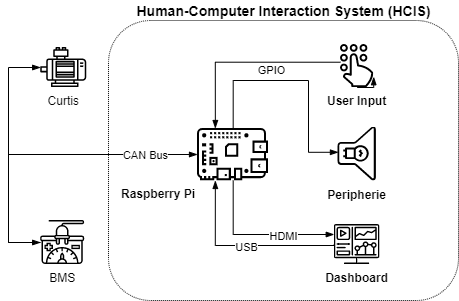
\includegraphics[scale=0.5]{figures/hcis/HCIS_Grundfunktion.png}
		\caption{Grundaufbau des Human-Computer Interaction Systems}
	\end{center}
\end{figure}

Nicht in der Abbildung dargstellt ist die Versorgung der einzelnen Komponenten, welche in dem folgenden Abschnitt noch genauer erläutert wird.
\subsection{Grundfunktionen des Systems}
Die geplanten Funktionen des HCIS lassen sich grob in vier Grundfunktionen einteilen.

\subsection{Zu bewältigende Aufgaben}


\section{Versorgung}
\section{Steuerung der Peripherie}
\section{Benutzeroberfläche}
\section{Kommunikation}
\section{Fahrdatenspeicher}